%Capitolo sulla logica predicativa e proposizionale nel corso Linguaggi di Programmazione
\chapter{Logica}
Effettuiamo ora un ripasso della logica proposizionale e predicativa, affrontata nel corso Fondamenti
dell'Informatica, al fine di rivedere e perfezionare i concetti necessari
per la comprensione e la scrittura di programmi logici.

Partiamo con l'esempio di una semplice dimostrazione geometrica:
\begin{teorema}
  Dato un triangolo isoscele (con $\overline{AB}=\overline{BC}$) si ha che $\angle A$ e $\angle C$, ovvero l'angolo in $C$, sono uguali.
\begin{figure}
\caption{Triangolo Isoscele}
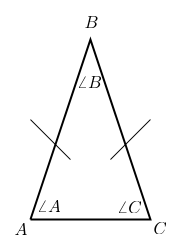
\includegraphics[scale=0.5]{img/tri.png}
\end{figure}
\end{teorema}
\begin{proof}

Si comincia la dimostrazione con l'elenco delle conoscenze pregresse:
\begin{enumerate}
\item se due triangoli sono uguali essi hanno lati e angoli uguali
\item se due triangoli hanno due lati e l'angolo sotteso uguale allora i due triangoli sono uguali
\item se viene definita la bisettrice di $\angle B$, $\overline{BH}$, si ha che $\angle ABH = \angle HBC$
\begin{figure}
\centering
\caption{Triangolo isoscele scomposto in due triangoli rettangoli}
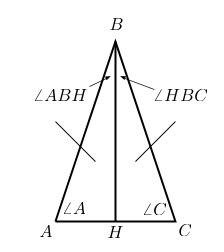
\includegraphics[scale=0.5]{img/tri2.png}
\end{figure}

\end{enumerate}
Procediamo ora coi passi della dimostrazione:
\begin{enumerate}
\item $\overline{AB}=\overline{BC}$ per ipotesi
\item $\angle ABH = \angle HBC$ per la terza conoscenza pregressa
\item $HBC = ABH$ per la seconda conoscenza pregressa in quanto due lati sono uguali per ipotesi e dal passo precedente
      l'angolo sotteso ai due lati uguali è uguale in ambedue i triangoli.
\item $\angle A= \angle C$ per la prima conoscenza pregressa dato che $HBC = ABH$
\end{enumerate}
Siamo così giunti alla fine della dimostrazione ma adesso vogliamo rappresentarla attraverso gli strumenti della logica al fine di renderla
totalmente formale per cui si effettua i seguenti passaggi:
\begin{itemize}
\item si è trasformata la seconda conoscenza pregressa in:\newline
  \textbf{se} $\overline{AB}=\overline{BC}$ \textbf{e} $\overline{BH}=\overline{BH}$ \textbf{e} $\angle ABH = \angle HBC$
  \textbf{allora} $ABH = HBC$
\item si è trasformata la prima conoscenza pregressa in:\newline
  \textbf{se} $ABH = HBC$ \textbf{allora} $\overline{AB}=\overline{BC}$ \textbf{e} $\overline{BH}=\overline{BH}$
  \textbf{e} $\overline{AH}=\overline{HC}$ \textbf{e} $\angle ABH = \angle HBC$ \textbf{e} $\angle AHB = \angle CBH$ \textbf{e} $\angle A=\angle C$
\end{itemize}
Possiamo ora procedere col processo di formalizzazione, ossia il processo che ci permette di affermare
$\overline{AB} = \overline{BC} \vdash \angle A = \angle C$ con $\vdash$ simbolo di derivazione logica.

Assumendo $P = \{ \overline{AB} = \overline{BC}, \angle ABH = \angle HBC, \overline{BH} = \overline{BH} \}$
ed avendo le seguenti conoscenze pregresse:
\begin{enumerate}
\item $\overline{AB}=\overline{BC} \land \overline{BH}=\overline{BH} \land \angle ABH = \angle HBC \rightarrow  ABH = HBC$
\item $ABH = HBC \rightarrow \overline{AB}=\overline{BC} \land \overline{BH}=\overline{BH} \land \overline{AH}=\overline{HC}
        \land \newline \angle ABH = \angle HBC \land \angle AHB = \angle CBH \land \angle A=\angle C$.
\end{enumerate}
per ottenere $\overline{AB} = \overline{BC} \vdash \angle A = \angle C$ bisogna effettuare la seguente catena:
\begin{description}
\item [P1] $\overline{AB}=\overline{BC}$  da \textbf{P}
\item [P2] $\angle ABH = \angle HBC$  da \textbf{P}
\item [P3] $\overline{BH}=\overline{BH}$  da \textbf{P}
\item [P4] $\overline{AB} = \overline{BC} \land \overline{BH} = \overline{BH} \land \angle ABH = \angle HBC$
       da \textbf{P1, P2, P3} attraverso l' \textbf{introduzione della congiunzione}.
\item [P5] $ABH = HBC$ da \textbf{P4}, dalla \textbf{regola 2}  attraverso l'applicazione del \textbf{modus ponens}.
\item [P6] $\overline{AB} = \overline{BC} \land \overline{BH} = \overline{BH} \land \overline{AH} = \overline{HC} \land \newline
  \angle ABH = \angle HBC \land \angle AHB = \angle CBH \land \angle A=\angle C$ da \textbf{P5}, dalla \textbf{regola 1} attraverso Modus Ponens.
\item [P7] $\angle A=\angle C$ da \textbf{P6} attraverso \textbf{eliminazione della congiunzione}
\end{description}
\end{proof}
\begin{defi}
  Una dimostrazione, chiamata \textbf{dim}, indicata con $S\,\,\vdash\,\, F$, è un sequenza:
\begin{equation*}
  dim=<P_1,P_2,...,P_n>
\end{equation*}
con:
\begin{itemize}
\item $P_n=F$
\item $P_i \in S$ o con $P_i$ ottenibile dalle $P_1,...,P_{i-1}$ applicando una regola di inferenza
\end{itemize}
\end{defi}
Un insieme di regole di inferenza costituisce la base di un calcolo logico, il quale ha lo scopo di manipolare le formule in modo
unicamente sintattico al fine di stabilire una connessione tra un insieme di formule di partenza, dette assiomi e un insieme di conclusioni.

\section{Logica Proporzionale}
La logica proposizionale si occupa delle conclusioni che si possono trarre da un insieme di proposizioni,
ma purtroppo è un linguaggio limitato in quanto non si può generalizzare le proposizioni e/o definire delle proprietà.

La sintassi di un linguaggio è composta da una serie di formule ben formate($FBF$) definite induttivamente nel seguente modo:
%definizione formule ben formate
\begin{enumerate}
  \item Le costanti e le variabili proposizionali sono $FBF$.
  \item Se $A$ e $B$ sono $FBF$ allora $(A \land B)$,$(A \lor B)$,$(\neg A)$,$(A \rightarrow B)$,
        $TA$ e $FA$ sono delle formule ben formate.
  \item nient'altro è una formula
\end{enumerate}

Esempio:\newline
$(P \land Q) \in Fbf$  è una formula ben formata\newline
$(PQ \land R) \not \in Fbf$ in quanto non si rispetta la sintassi del linguaggio definita.\newline

La semantica di una logica consente di dare un significato e un interpretazione alle formule del Linguaggio.\newline
\begin{defi}
  Sia data una formula proposizionale $P$ e sia ${P_1,\dots,P_n}$, l'insieme degli atomi che compaiono nella formula $A$.\newline
  Si definisce come \emph{interpretazione} una funzione $v:\{P_1,\dots,P_n\} \mapsto \{T,F\}$ che attribuisce un valore di verità
  a ciascun atomo della formula $A$.
\end{defi}
I connettivi della Logica Proposizionale hanno i seguenti valori di verità:
%Tabella di Verità degli operatori
\begin{table}
$\begin{array}{cccccc}
\toprule
\text{A} & \text{B} & A \land B & A \lor B & \neg A & A \rightarrow B\\
\midrule
    F & F & F & F & T & T\\
    F & T & F & T & T & T\\
    T & F & F & T & F & F\\
    T & T & T & T & F & T\\
\bottomrule
\end{array}$
\end{table}
La tavola di verità costituisce la semantica di un insieme di proposizioni mentre un calcolo logico dice come generare nuove formule logiche,
ovvero espressioni sintattiche, a partire dagli assiomi e questo processo di generazione si chiama dimostrazione.

Per ottenere nuove formule dagli assiomi si usa il calcolo proposizionale, che si base sulle regole di inferenza, ossia regole attraverso
cui si può derivare una nuova formula ben formata.\newline
Le regole di inferenza analizzate sono le seguenti:
\begin{itemize}
\item \textbf{Modus Ponens:}
  \begin{equation*}
    \frac{a\to b,\,\,a}{b}
  \end{equation*}
\item \textbf{Modus Tollens:}
  \begin{equation*}
    \frac{a\to b, \neg b}{\neg a}
  \end{equation*}
\item \textbf{Eliminazione $\land$:}
  \begin{equation*}
    \frac{P_1\land P_2 \land ... \land P_n}{P_i}\,\,
  \end{equation*}
\item \textbf{Introduzione di $\land$}:
  \begin{equation*}
    \frac{P_1, P_2,...,P_n}{P_1\land P_2 \land ... \land P_n}\,\,
  \end{equation*}
\item \textbf{Introduzione di $\lor$:}
  \begin{equation*}
    \frac{a}{a \lor b}
  \end{equation*}
\item \textbf{Terzo Escluso:}
  \begin{equation*}
    \frac{a \lor \neg a}{vero}
  \end{equation*}

\item \textbf{Eliminazione di $\neg$}:
  \begin{equation*}
    \frac{\neg \neg a}{a}
  \end{equation*}

\item \textbf{Eliminazione di $\land$}:
  \begin{equation*}
    \frac{a \land vero}{a}
  \end{equation*}
\item \textbf{Contraddizione:}
  \begin{equation*}
    \frac{a \land \neg a}{b}
  \end{equation*}
ovvero da una contraddizione posso trarre qualsiasi conseguenza
\end{itemize}
Queste regole di inferenza fanno parte del calcolo naturale, detto anche di Gentzen, similare al calcolo tramite Tableaux visto nel corso
di Fondamenti dell'informatica.\newline
Questo tipo di calcolo consiste nel formalizzare i modi di derivare conclusioni a partire dalle premesse, ovvero di derivare direttamente un FBF
mediante una sequenza di passi ben codificati.\newline
La regola del modus ponens  insieme al principio del terzo escluso, posso essere usati anche procedendo per assurdo alla dimostrazione
di una data formula e ciò viene detto \emph{principio di risoluzione}, affrontata poi quando analizziamo il linguaggio Prolog.

Una formula nella logica proposizionale può essere di 4 diversi tipi:
%Tipologie di formule
\begin{description}
    \item[tautologica] la formula è soddisfatta da qualsiasi valutazione della formula.
    \item[soddisfacibile non tautologica] la formula è soddisfatta da qualche valutazione.
    \item[falsibicabile] la formula non è soddisfatta da qualche valutazione della formula.
    \item[contraddizione] la formula non viene mai soddisfatta.
\end{description}

La logica proposizionale è decidibile, ossia posso sempre verificare il significato di una formula, infatti esiste
una procedura effettiva che stabilisce la validità o no di una formula, o se questa ad esempio è una tautologia.\newline
In particolare il verificare se una proposizione è tautologica o meno è l’operazione di decibilità principale che si svolge
nel calcolo proposizonale.

Una dimostrazione di una formula di una logica può venire tramite:
\begin{itemize}
  \item  \textbf{Metodo diretto}: Data un'ipotesi, attraverso una serie di passi
          si riesce a dimostrare la correttezza della Tesi
  \item \textbf{Metodo per assurdo}(non sempre accettato in tutte le logiche):
        Si nega la tesi ed attraverso una serie di passi si riesce a dimostrare
        la negazione delle ipotesi.
\end{itemize}

La logica proposizionale è completa e corretta per cui data una formula ben formata, sia utilizzando i sistemi deduttivi sia analizzando
la semantica, si è in grado di stabilire se una formula è tautologica, soddisfacibile o falsificabile.

\section{Logica del primo ordine}
La logica del primo ordine, chiamata anche logica predicativa, permette di quantificare i vari fatti ed introduce il concetto di funzione e
predicato per poter esprimere delle proprietà su una serie di individui.

Un linguaggio predicativo $L$ è composto dai seguenti insiemi di simboli:
\begin{enumerate}
    \item insieme di variabili individuali(infiniti) $x,y,z,\dots$
    \item connettivi logici: $\land \lor \neg \rightarrow \iff$
    \item quantificatori: $\forall \exists$
    \item simboli: ( , )
    \item Costanti proposizionali: $T,F$
    \item simbolo di uguaglianza $=$, eventualmente assente
\end{enumerate}
Questa è la parte del linguaggio tipica di ogni linguaggio del primo ordine poi ogni linguaggio definisce la propria segnatura:
\begin{enumerate}
    \item insiemi di simboli di costante $a,b,c,\dots$
    \item simboli di funzione con arieta $f,g,h,\dots$
    \item simboli di predicato $P,Q,Z,\dots$ con arietà
\end{enumerate}

%Esempio
Esempio:Linguaggio della teoria degli insiemi \newline
Costante:$\emptyset$\newline
Predicati:$\in(x,y)$, $=(x,y)$

Esempio:Linguaggio della teoria dei Numeri \newline
Costante:$0$ \newline
Predicati:$<(x,y)$,$=(x,y)$ \newline
Funzioni:$succ(x)$,$+(x,y)$,$*(x,y)$

%Definizione di Termini e Formule ben formate
Per definire le formule ben formate della logica predicativa bisogna prima definire
l'insieme di termini e le formule atomiche.
\begin{defi}
    L'insieme $TERM$ dei termini è definito induttivamente come segue
    \begin{enumerate}
        \item Ogni variabile e costante è un termine
        \item Se $t_1 \dots t_n$ sono dei termini e $f$ è un simbolo di funzione di arietà $n$
              allora $f(t_1,\dots,t_n)$ è un termine
    \end{enumerate}
\end{defi}
%Inserire esempi
\begin{defi}
    L'insieme $ATOM$ delle formule atomiche è definito come:
    \begin{enumerate}
        \item $T$ e $F$ sono degli atomi
        \item Se $t_1$ e $t_2$ sono dei termini, allora $t_1 = t_2$ è un atomo
        \item Se $t_1,\dots,t_n$ sono dei termini e $P$ è un predicato a $n$ argomenti,
              allora $P(t_1,\dots,t_n)$ è un atomo.
    \end{enumerate}
\end{defi}
%Inserire esempi
\begin{defi}
    L'insieme delle formule ben formate($FBF$) di $L$ è definito induttivamente come
    \begin{enumerate}
        \item Ogni atomo è una formula
        \item Se $A,B \in FBF$, allora $\neg A$, $A \land B$,$A \lor B$,$A \rightarrow B$
              e $A \iff B$ appartengono alle formule ben formate
        \item Se $A \in FBF$ e $x$ è una variabile, allora $\forall x A$ e $\exists x A$
              appartengono alle formule ben formate
        \item Nient'altro è una formula
    \end{enumerate}
\end{defi}
%Inserire esempi

%Variabili legate e chiuse
\begin{defi}
    L'insieme $var(t)$ delle variabili di un termine $t$ è definito come segue:
    \begin{itemize}
        \item $var(t) = \{t \}$, se $t$ è una variabile
        \item $var(t) = \emptyset$ se $t$ è una costante
        \item $var(f(t_1,\dots,t_n)) = \bigcup _{i = 1} ^n var(t_i)$
        \item $var(R(t_1,\dots,t_n)) = \bigcup _{i = 1} ^ n var(t_i)$
    \end{itemize}
\end{defi}
Si definisce come \emph{aperto} un termine che non contiene variabili altrimenti il termine è \emph{chiuso}.\newline
Le variabili nei termini e nelle formule atomiche possono essere soltanto libere
in quanto gli unici operatori che "legano" le variabili sono i quantificatori.

Il campo di azione dei quantificatori si riferisce soltanto alla parte in cui si applica il quantificatore per cui
una variabile si dice \emph{libera} se non ricade nel campo di azione di un quantificatore altrimenti è \emph{vincolata}.

Si aggiunge una nuova regola d'inferenza per la logica dei predicati, l'eliminazione del quantificatore universale $\forall$:
\begin{equation*}
  \frac{\forall x, T(...,x,...), c\in C}{T(...,c,...)}
\end{equation*}

Abbiamo altre regole di inferenza per il quantificatore esistenziale:
\begin{itemize}
\item \textbf{Introduzione del quantificatore esistenziale $\exists$}:
  \begin{equation*}
    \frac{T(...,c,...), c\in C}{\exists x, T(...,x,...)}
  \end{equation*}
\item si hanno le seguente identità:
  \begin{equation*}
    \begin{split}
      \exists x, \neg T(...,x,...)\equiv \neg\forall x, T)...,x,...) \\
      \forall x, \neg T(...,x,...)\equiv \neg\exists x, T(...,x,...)\\
    \end{split}
  \end{equation*}
\end{itemize}
Per una trattazione migliore e per approfondimenti sulla logica si può consultare gli appunti del corso di Fondamenti oppure i vari libri di
logica, come ad esempio ``How to prove it''.
